
\subsection{Certification Perspective}
%\addcontentsline{toc}{subsection}{Certification Perspective}

Data security and data sovereignty are the fundamental value propositions of the International Data Spaces. Data sovereignty can be defined as a natural person’s or legal entity’s capability of being in full control of its data. Therefore, any organization or individual seeking permission to access the International Data Spaces is certified, and so are the core software components (e.g., the IDS Connector) the participants use to securely exchange data with one another While the certification of organizations and individuals focuses on security and trust, the certification of components also refers to compliance with technical requirements ensuring interoperability.


To ensure a consistent process in the certification of participants and core components, the IDS uses a Certification Scheme comprising all processes, rules, and standards governing the certification process. The IDS Certification Scheme follows best practices from other, internationally accredited certification concepts. 



\subsubsection{Certification Aspects Addressed by the Different Layers of the IDS-RAM}
%\addcontentsline{toc}{subsubsection}{Certification Aspects Addressed by the Different Layers of the IDS-RAM}
\paragraph{Business Layer\\}

The Certification Body and the Evaluation Facility are in charge of the certification process. Their interactions and responsibilities in this process are described in section 4.2.2.


Organizations assuming a role under one of the three categories Core Participant, Intermediary, and Software/Service Provider (see Section 3.1.1) are potential targets of certification. The IDSA Whitepaper Certification\footnote{ IDSA White Paper Certification – Framework for the IDS Certification Scheme, Version 2.0 https://www.internationaldataspaces.org/publications/whitepaper-certification/ } describes for each role what level of certification is required and what the focus of the certification is.


\paragraph{Functional Layer\\}
The functional requirements of the International Data Spaces are the core requirements expected to be implemented by the technical core components (e.g., the Connector or the Clearing House). Therefore, compatibility of each such implementation with these functional requirements forms the basis of the compliance part of a core component’s certification. The security part of the certification focuses on security specific requirements. As for the Security Perspective (see Section 4.1), these security specific requirements are mainly related to the System Layer.

\paragraph{Process Layer\\}
Whenever relevant for the compliance part of a component’s certification, a component is also evaluated in terms of whether it fully supports all processes it is involved in, as defined by the Reference Architecture Model.

\paragraph{Information Layer\\}
Certification of a core component comprises also its compliance with the Reference Architecture Model regarding functionality, protocols, etc. Whenever relevant, evaluation of a core component’s compliance also refers to its compatibility with the Information Model defined at the Information Layer.

\paragraph{System Layer\\}
The System Layer defines the possible interactions between the components, detailed requirements for the Connector, and specific types of Connector implementations. The System Layer is the predominant layer regarding the security part of a component’s certification.



\subsubsection{Certification Process }
%\addcontentsline{toc}{subsubsection}{Certification Process }

Figure \ref{fig:Certification_process} outlines the basic structure of the certification process, together with the roles involved in this process. The Certification Body and the Evaluation Facility belong to the $``$Governance Body$"$  category specified on the Business Layer (see section 3.1.1). The tasks of these roles with regard to the certification process are outlined in the following paragraphs. An in-depth description of their responsibilities can be found in Part 1 of the White Paper Certification\footnote{ IDSA White Paper Certification – Framework for the IDS Certification Scheme, Version 2.0 https://www.internationaldataspaces.org/publications/whitepaper-certification/ }.


It should be noted that all roles described in this section are specific to the International Data Spaces (i.e. terms such as $``$Certification Body$"$  should not be misunderstood to refer to an existing organization already granting certificates).



%%%%%%%%%%%%%%%%%%%% Figure/Image No: 63 starts here %%%%%%%%%%%%%%%%%%%%

\begin{figure}[H]
	\begin{Center}
		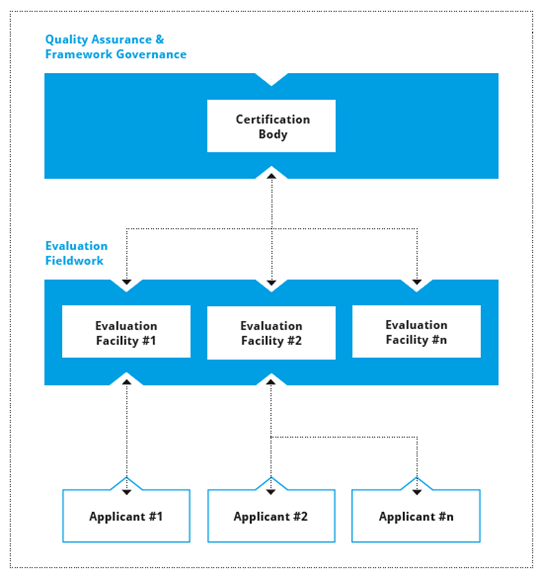
\includegraphics[width=5.63in,height=5.98in]{./media/image79.png}
		\caption{Certification process}
		\label{fig:Certification_process}
	\end{Center}
\end{figure}


%%%%%%%%%%%%%%%%%%%% Figure/Image No: 63 Ends here %%%%%%%%%%%%%%%%%%%%



\paragraph{Certification Body \\}
The Certification Body oversees the certification process regarding quality assurance and framework governance. It defines standard evaluation procedures and supervises the actions of the Evaluation Facilities. A certificate is granted only if both the Evaluation Facility and the Certification Body have come to the conclusion that all preconditions for certification are fulfilled.

\paragraph{Evaluation Facility \\}
Contracted by an Applicant (see below), the Evaluation Facility is responsible for carrying out the detailed technical and/or organizational evaluation work during a certification process. The Evaluation Facility issues an evaluation report for the respective organization/individual or core component, listing details regarding the evaluation process as well as information regarding the confirmed security level (the latter determines the depth and scope of the evaluation activities performed).

The term $``$Evaluation Facility$"$  refers both to authorized auditors for management system evaluations (i.e., for participant certifications) as well as approved evaluators for product evaluations (i.e., for core component certifications). Hence, the Certification Body oversees and cooperates with multiple Evaluation Facilities. However, in each evaluation of an organization/individual or core component only one Evaluation Facility is involved.

\paragraph{Applicant \\}
The Applicant is not just the subject of the evaluation and certification process, but plays an active part in it.

An Applicant needs to actively submit an application to trigger the certification process. This applies to organizations/individuals that develop software components intended to be deployed within the International Data Spaces (i.e., prospective Software Providers) and to organizations that intend to become IDS Participants.

\paragraph{Certification Process \\}
The certification process is divided into the following three phases:

\begin{enumerate}
	\item Application Phase: The main goal of this stage is the successful start of the IDS evaluation and certification process.

	\item Evaluation Phase: The main goal of this stage is the evaluation of an applicant or core component based on the defined evaluation criteria.

	\item Certification Phase: The main goal of this stage is the examination of the evaluation report by the certification body, which issues a certificate if the result of the evaluation process is positive.

\end{enumerate}

After a successfully completed evaluation process, the Certification Body awards an International Data Spaces certificate to the applicant. This certificate has a limited validity period. In order to renew a certificate before it expires, re-certification is required, taking into account any relevant external developments that have happened in the meantime. Similarly, re-certification is required if changes are made to the target of certification.


For authentication and authorization, each IDS component must have a valid X.509 certificate. These technical certificates digitally represent the evaluation certificate and enable automated trust checks between partners prior to data transfer within the International Data Spaces.


A more detailed description of the phases and the issuing of digital certificates can be found in Part 1 and 4 of the White Paper Certification\footnote{ IDSA White Paper Certification – Framework for the IDS Certification Scheme, Version 2.0 https://www.internationaldataspaces.org/publications/whitepaper-certification/ }.


\subsubsection{Certification of Participants and Core Components}
%\addcontentsline{toc}{subsubsection}{Certification of Participants and Core Components}
\paragraph{Participant Certification \\ }

Participants in the International  Data Spaces collaborate by exchanging and sharing valuable data. For this collaboration, the IDS provides a trusted business ecosystem. Furthermore, it is essential for the  International  Data Spaces and its reputation that the participants themselves are trustworthy. This is achieved by evaluating each participant regarding fulfilment of defined levels of security, including infrastructure reliability and process compliance. 


To build this trust in a structured way, the International Data Spaces has established a well-defined process for participant certification. An in-depth description of the certification process (also with regard to each role) can be found in Part 2 of the White Paper Certification\footnote{ IDSA White Paper Certification – Framework for the IDS Certification Scheme, Version 2.0 https://www.internationaldataspaces.org/publications/whitepaper-certification/ }. The participant certification criteria catalog is available for free to all IDSA members. \par


\paragraph{Core Component Certification \\}

Core components to be used in the IDS must provide the required functionality and level of security. The certification of core components focuses on interoperability and security, while aiming to strengthen the development and maintenance process of these components.

To build this trust in a structured way, the International Data Spaces has established a well-defined process for core component certification. An in-depth description of the certification process, and how it applies to the key elements of the IDS architecture, can be found in Part 3 of the White Paper Certification\footnote{IDSA White Paper Certification – Framework for the IDS Certification Scheme, Version 2.0 https://www.internationaldataspaces.org/publications/whitepaper-certification/ }. The core component certification criteria catalogue is available for free to all IDSA members.
